\documentclass[a4paper, 10pt]{article}
\usepackage[a4paper,top=1in,bottom=1in,left=1in,right=1in]{geometry}

% Chemfig
\usepackage{chemfig}

% Tabularx
\usepackage{tabularx}

% Tikz package for diagramming
\usepackage{tikz}

% Fancyhdr for a fancy header!
\usepackage{fancyhdr}
\setlength{\headheight}{1em}
\pagestyle{fancyplain}
\lhead{BIOL6300 - Biochemistry}
\chead{Sanger Sequencing}
\rhead{\today}

% No paragraph indents, spacing between paragraphs of 1em
\setlength{\parindent}{0cm} % Default is 15pt.
\setlength{\parskip}{1em}

% define new command to add degree symbol
\newcommand{\degree}{\ensuremath{^\circ}}

\begin{document}

\definesubmol{ribose}{{^-}O-P(-[2]O\rlap{${}^-$})(=[6]O)(-O-CH_2(-[2,.25,,,draw=none]\scriptstyle\color{red}{5'})-[6]?([7,.7]<(-[2,.4]H)(-[6,.4]OH)(-[1,.25,,,draw=none]\scriptstyle\color{red}3')-[0,.7,,,line width=2pt](-[2,.4]H)(-[6,.4,,,red]\color{red}{OH})>[1,.7](-[6,.4]H-[2,2.5]\framebox{Purine or pyrimidine base})-[:150,.95]O?)-[6]H)}

\definesubmol{deoxyribose}{{^-}O-P(-[2]O\rlap{${}^-$})(=[6]O)(-O-CH_2(-[2,.25,,,draw=none]\scriptstyle\color{red}{5'})-[6]?([7,.7]<(-[2,.4]H)(-[6,.4]OH)(-[1,.25,,,draw=none]\scriptstyle\color{red}3')-[0,.7,,,line width=2pt](-[2,.4]H)(-[6,.4,,,red]\color{red}{H})>[1,.7](-[6,.4]H-[2,2.5]\framebox{Purine or pyrimidine base})-[:150,.95]O?)-[6]H)}

\definesubmol{dideoxyribose}{{^-}O-P(-[2]O\rlap{${}^-$})(=[6]O)(-O-CH_2(-[2,.25,,,draw=none]\scriptstyle\color{red}{5'})-[6]?([7,.7]<(-[2,.4]H)(-[6,.4,,,red]\color{red}{H})(-[1,.25,,,draw=none]\scriptstyle\color{red}3')-[0,.7,,,line width=2pt](-[2,.4]H)(-[6,.4,,,red]\color{red}{H})>[1,.7](-[6,.4]H-[2,2.5]\framebox{Purine or pyrimidine base})-[:150,.95]O?)-[6]H)}

\begin{tabularx}{\linewidth}{cc}
\setcrambond{2pt}{}{}
\chemname{\chemfig{!{deoxyribose}}}{\textbf{Deoxyribose}} &
\setcrambond{2pt}{}{}
\chemname{\chemfig{!{dideoxyribose}}}{\textbf{2{$'$},3{$'$}Dideoxyribose}} \\
\end{tabularx}

\begin{enumerate}
\item A single stranded DNA template, a DNA primer, DNA polymerase, normal dNTPs and ddNTPs.
\item Heat denature DNA and add primer and polymerase, in order to purify template DNA.
\item Add 1\% mixtures of ddATP, ddTTP, ddCTP, ddGTP to 4 separate mixtures (1 per well.)
\item Add polymerase to each of the 4 mixtures.
\item Newly polymerized sequences will have varying lengths, based on where ddNTP was inserted.
\item Heat denature and place sequences in polyacrylamide gel and perform electrophoresis, short sequences migrate faster towards the positive anode placed at the bottom of the gel (due to the negative net charge of DNA.)
\item Gel will now have a series of bands, sorted by length, corresponding to the DNA sequence.
\item Reading the bands from bottom to top yields the sequence.
\end{enumerate}

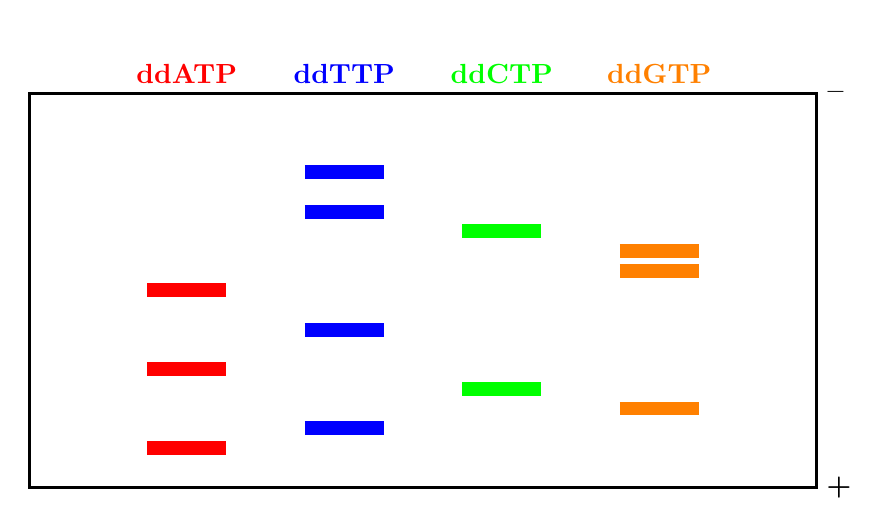
\begin{tikzpicture}
\draw [very thick] (0,0) rectangle (10,5) [right] node{\textbf{--}};
\draw (10,0) [right] node{\textbf{+}};

% Well labels
\draw (2,5) [red, above] node{\textbf{ddATP}};
\draw (4,5) [blue, above] node{\textbf{ddTTP}};
\draw (6,5) [green, above] node{\textbf{ddCTP}};
\draw (8,5) [orange, above] node{\textbf{ddGTP}};

% A
\draw [red, line width=5] (1.5,0.5) -- (2.5,0.5);
\draw [red, line width=5] (1.5,1.5) -- (2.5,1.5);
\draw [red, line width=5] (1.5,2.5) -- (2.5,2.5);
\draw [red, line width=5] (1.5,0.5) -- (2.5,0.5);
% T
\draw [blue, line width=5] (3.5,0.75) -- (4.5,0.75);
\draw [blue, line width=5] (3.5,2) -- (4.5,2);
\draw [blue, line width=5] (3.5,3.5) -- (4.5,3.5);
\draw [blue, line width=5] (3.5,4) -- (4.5,4);
% C
\draw [green, line width=5] (5.5,1.25) -- (6.5,1.25);
\draw [green, line width=5] (5.5,3.25) -- (6.5,3.25);

% G
\draw [orange, line width=5] (7.5,1) -- (8.5,1);
\draw [orange, line width=5] (7.5,2.75) -- (8.5,2.75);
\draw [orange, line width=5] (7.5,3) -- (8.5,3);
\end{tikzpicture}

Here we can see the sequence represented is:\\\\

\begin{tikzpicture}
\draw [red] (1.5,0.25) |- (2,0) -| (2.5,0.25);
\draw (2,0) [midway, above] node{ATG};
\draw [red] (3.5,0.25) |- (4,0) -| (4.5,0.25);
\draw (4,0) [midway, above] node{CAT};
\draw [red] (5.5,0.25) |- (6,0) -| (6.5,0.25);
\draw (6,0) [midway, above] node{AGG};
\draw [red] (7.5,0.25) |- (8,0) -| (8.5,0.25);
\draw (8,0) [midway, above] node{CTT};
\end{tikzpicture}

Next-gen sequencing is performed in a similar fashion, except that instead of radio-nucleotides, we use fluorescent ddNTP nucleotides all in a single capillary.  The fluorescent pattern is then read with a laser detector and a color profile emerges, yielding the sequence.\\
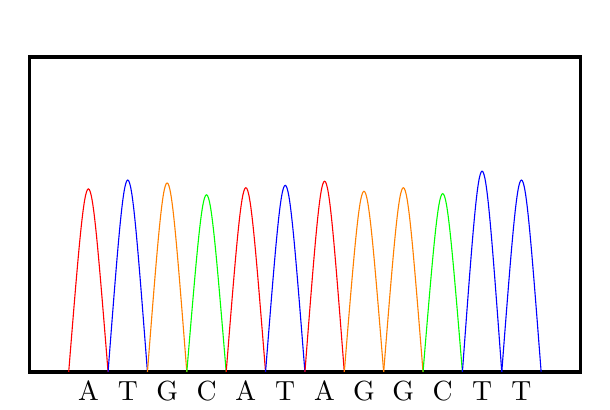
\begin{tikzpicture}
\draw [very thick] (0,0) rectangle (7,4);

\draw [red] (0.5,0) .. controls (0.75,3.1) .. (1.0,0);
\draw (0.75,0) [below] node {A};

\draw [blue] (1.0,0) .. controls (1.25,3.25) .. (1.5,0);
\draw (1.25,0) [below] node {T};

\draw [orange] (1.5,0) .. controls (1.75,3.2) .. (2.0,0);
\draw (1.75,0) [below] node {G};

\draw [green] (2.0,0) .. controls (2.25,3) .. (2.5,0);
\draw (2.25,0) [below] node {C};

\draw [red] (2.5,0) .. controls (2.75,3.12) .. (3.0,0);
\draw (2.75,0) [below] node {A};

\draw [blue] (3.0,0) .. controls (3.25,3.16) .. (3.5,0);
\draw (3.25,0) [below] node {T};

\draw [red] (3.5,0) .. controls (3.75,3.23) .. (4.0,0);
\draw (3.75,0) [below] node {A};

\draw [orange] (4.0,0) .. controls (4.25,3.06) .. (4.5,0);
\draw (4.25,0) [below] node {G};

\draw [orange] (4.5,0) .. controls (4.75,3.12) .. (5.0,0);
\draw (4.75,0) [below] node {G};

\draw [green] (5.0,0) .. controls (5.25,3.02) .. (5.5,0);
\draw (5.25,0) [below] node {C};

\draw [blue] (5.5,0) .. controls (5.75,3.4) .. (6.0,0);
\draw (5.75,0) [below] node {T};

\draw [blue] (6.0,0) .. controls (6.25,3.25) .. (6.5,0);
\draw (6.25,0) [below] node {T};
\end{tikzpicture}

\end{document}